\chapter{Previous Work}\label{chap:litReview}

Laureti et al. \cite{laureti2006information} introduced IF as an aggregation method. Its original layout appropriated methods that examined complex networks within the community and applied them to scoring systems on the internet. From this, it was established found that a reciprocal variance method was successful at reducing the effects of systemic errors and collusion. Primarily concerned with the case of voting on the internet, it was demonstrated that the reciprocal variance weighting system described in equation \ref{eq:negRecip} reduced the effectiveness of a cheater the more they cheated. This is demonstrated in figure \ref{fig:recipCheating}.

\begin{figure}[H]
    \centering
    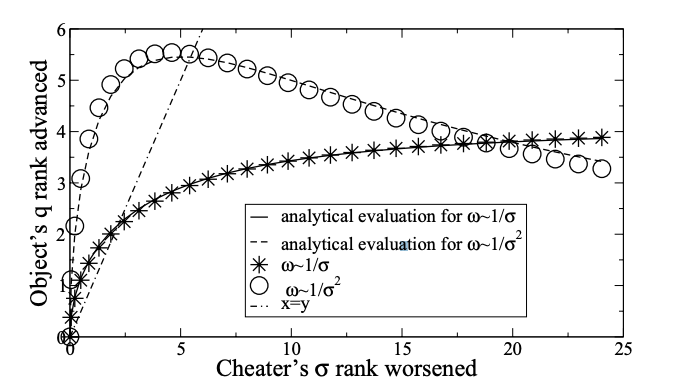
\includegraphics{Figures/recipCheating.png}
    \caption[Relationship between voters accuracy and marginal effect of their vote on an object]{Relationship between voters accuracy and marginal effect of their vote on an object, from \textcite{laureti2006information}.}
    \label{fig:recipCheating}
\end{figure}

De Kerchoove and Van Dooren \cite{de2007iterative} went on to improve the applicability of the algorithm by examining a variety of weighting functions, including the affine method defined recursively in equations \ref{eq:affine} and \ref{eq:affineBase}. This was explored to account for predictable human behaviours, such as clumsiness or dishonesty. This was achieved by augmenting the MovieLens dataset with a group of random voters and a group that colluded to increase the ratings of a set of movies. Both groups were shown to have significantly reduced trust ratings compared to real voters.
Progressing forward, this study conceptualised the application of IF in dynamical systems (i.e. one where the set of ratings and raters are non-stationary over time). The examination of such a system is particularly relevant to the topic of this thesis. However the lack of examination in ratings degradation to preempt changes in quality over time, prevents the full realisation of the scope of this project to be achieved. Despite this, the experiments conducted validated a slightly modified\footnote{Limiting the number of iterations rather than continuing until convergence was found to provide adequate results while still allowing for rapid updates of ratings.} reciprocal variance method for use within dynamical systems. Through a number of other experiments De Kerchoove and Van Dooren proved that IF is very useful for cheater detection. 

\begin{align}
    \tilde{u}^{(n)} &= \sum\limits_{i \in R}\frac{\frac{r_i}{|r_i-\tilde{u}^{(n-1)}|+\epsilon}}{\sum\limits_{j\in R} \frac{1}{|r_j-\tilde{u}^{(n-1)}|+\epsilon}} \label{eq:affine} \\
    \tilde{u}^{(0)} &= \frac{\sum\limits_{i\in R} r_i}{|R|}\label{eq:affineBase}
\end{align}


De Kerchoove and Van Dooren's \cite{de2010iterative} second paper in the area went into great detail regarding the mathematical properties of the various quadratic and affine weighting methods available. It explained and demonstrated the validity of all of the methods specified in table \ref{tab:deKerchWeight}. The paper goes on to examine the effects of a very sparse voting matrix. Noting that even extreme sparsity does not invalidate any of the ideal properties of the examined algorithms, including robustness against cheating or randomness. Furthermore, the paper demonstrates the effectiveness of modified techniques, such as specifying various constants (specifically increasing $k$ as seen in table \ref{tab:deKerchWeight}), in aggregating such sparse information.

\begin{table}[H]
    \centering
    \begin{tabular}{c c}
    \toprule\toprule
    Weighting System & Formula of Weight \\ \midrule
    Reciprocal Variance & $\frac{1}{\sigma^2}$ \\
    \addlinespace
    Reciprocal Standard Deviation & $\frac{1}{\sigma}$\\
    \addlinespace
    Exponential & $e^{-kd}$ \\
    \addlinespace
    Affine & $1-kd$ \\ \bottomrule
    \end{tabular}
    \caption[Common IF weighting systems]{Common IF weighting systems examined by De Kerchoove and Van Dooren \cite{de2010iterative}, with $d$ refering to absolute distance between a rating and the calculated mean and $k$ being a constant}
    \label{tab:deKerchWeight}
\end{table}

These techniques will likely be very useful when designing a system that observes recommendations regarding small-cap stocks which are typically under-covered by analysts. By ensuring that the method chosen is valid for all securities, the system could be more easily expanded and automated for a larger range of financial products.

Zhou et al. \cite{zhou2011robust} adds to the current set of quadratic and affine weighting paradigms by designing a system that correlated a user's and objects rating to enhance it's assignment of weights (seen in equation \ref{eq:qbullshit}). This method was shown to be very effective in aggregating datasets with a high ratio of spammers however did not perform as well as other algorithms in datasets with a lower ratio. Depending on the quantity of analysts with no significant skill this method may be quite useful.


\begin{equation}
    \tau_i = max\left(0, 
    \frac{1}{|j:i\rightarrow j|}
    \sum\limits_{j:i\rightarrow j}
    \left(\frac{r_{i,j} - \bar{r}_i}{\sigma_{r_i}}\right)
    \left(\frac{v_{j} - \bar{v}_{j:i\rightarrow j}}{\sigma_{v_{j:i\rightarrow j}}}\right)
    \right) \label{eq:qbullshit}
\end{equation}

Ignjatovic et al. \cite{ignjatovic2009computing} specifically examines the case of multiple assessors marking assignments. This model works to suggest parameter modifications for issues that are likely to be encountered in said scenario. Mainly these adjustments are made if there exists a strong presence of systematic bias or there is a small number of markers per assessment. This working theory is also represented in the problem at hand where the number and frequency of recommendations is likely to correlate quite strongly with the market cap of the stock. Thus a system that accounts for these issues when aggregating ratings will be able to provide more valid recommendations.

Rezvani et al. \cite{rezvani2018provenance} utilises several modification sand adaptations of existing methods to explore the concept of provenance, i.e. external factors that could be used to augment trust ratings. Potential factors that might aid in producing more valid results are explored in section \ref{sec:plan}.

The literature in the area has produced multiple techniques that will aid significantly in the development of an algorithm to aggregate financial data. This signifies that approaches for dynamical systems, sparse voting patterns, issues of collusion and bias, and accounting for provenance can be specified and validated. In order to incorporate these techniques, several procedures that aren't addressed by literature will need to be investigated. Namely, this refers to the formulation of a method that considers the combined effect that of sparsity, white noise, and systematic bias has on financial data. This will result in a trust system that expects, rather than allowing for, changes in the quality of a reviewer, as well as methods for deriving provenance factors.